% Generated using vi
% Author: Dominic van der Zypen
% Last modified 2013-10-08

\documentclass[11pt, a4paper]{amsart}
\usepackage{a4wide}
\usepackage{amssymb}
\usepackage{amsthm}
\usepackage{amsfonts}
\usepackage{tikz}
\newtheorem{lemma}{\bf Lemma}[section]
\newtheorem{theorem}[lemma]{\bf Theorem}
\newtheorem{corollary}[lemma]{\bf Corollary}
\newtheorem{proposition}[lemma]{\bf Proposition}
\newtheorem{fact}[lemma]{\bf Fact}
\newtheorem{definition}[lemma]{\bf Definition}
\newtheorem{example}[lemma]{\bf Example}
\newcommand{\restrict}{\mbox{$\mid$}}
\newcommand{\Pow}{{\mathcal P}}
\newcommand{\Pz}{{\mathcal P}_2}
\newcommand{\card}{{\mathrm{card}}}
\newcommand{\ascii}{{\mathtt{ascii}}}

\begin{document}

%...... title
\title{Rolling XOR hash for Rabin-Karp}

%...... authors
\author{Marcel L\"uthi, Stefanie Neuhaus, Dominic van der Zypen}
%\address{Swiss Armed Forces, CH-3003 Bern, Switzerland}
%\email{dominic.zypen@protonmail.ch}

%......MSC subject class
\subjclass[2010]{05C15, 05C83}

%...... Abstract...
\begin{abstract} We present a very simple, rolling XOR-based 
hash function that is much faster than other established hash functions
in the application of the Rabin-Karp string-searching algorithm.
\end{abstract}

%....... main()
\maketitle
\parindent = 0mm
\parskip = 2 mm
% . . . . . . . . . . . . . . . . .
\section{Introduction}
The Rabin-Karp algorithm \cite{RK} is a string-searching algorithm created by 
Richard Karp and Michael Rabin in 1987 that uses hashing instead of letter-to-letter
comparison to find an exact match of a pattern in a text. Rabin-Karp calculates 
the hash of the pattern once, and then has a ``text window'' of the same length as the 
pattern stepping through the text. At each position the hash of the 
window is calculated and compared to the the hash of the pattern. If the
hashes are equal, a match is declared to be found. False negatives cannot 
occur by construction, but there may be false positives.

Execution time depends on the (rolling) hash used. Here we present a 
rolling hash that only uses bitwise XOR ($\oplus$ in mathematical notation;
\string^ in the programming language {\tt C}, {\tt Go}, and others).


% . . . . . . . . . . . . . . . . .
\section{XOR wrap hash}
We first construct a very simple  
hash function that is reminiscent of Pearson hashing. For our 
purposes, we hashed to 64 bits ({\tt uint64\_t} in C), but 
the algorithm can easily be adapted to any bit number that 
is a multiple of $8$.

For the following, note that a 64bit integer consists of 8 bytes.

Start with hash value ${\tt h = 0}$, and from the string {\tt s[]} 
to be hashed copy the first character\footnote{{\tt char} in C; 
given as byte of 8 bit} into the 8 least significant bytes of {\tt h}. Copy the next
character of {\tt s[]} into the next 8 bits of {\tt h}.

The 9th character ({\tt s[8]}) gets XOR'ed with the 8 least significant 
bits in {\tt h} (where {\tt s[0]} was stored before), and we XOR 
{\tt s[9]} with the next 8 bits of {\tt h} and so on. In other words, we ``wrap'' 
{\tt s[]} around {\tt h} as is shown in the following example.


\begin{example}
We are hashing the string {\tt hello world} to demonstrate
the wrapping mechanism.
\begin{center}
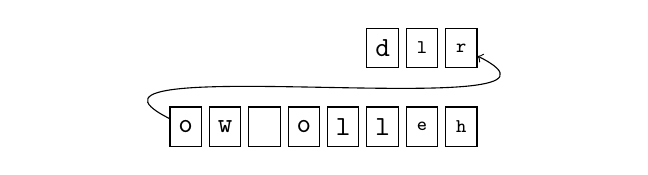
\begin{tikzpicture}[
   box/.style={rectangle,draw,minimum width=0.4cm,
    minimum height=0.5cm,inner sep=+0.1cm}
    ]
    
  % -- bottom row
  \node[box] at (1,0) (b7) {\tt o};
  \node[box] at (1.5,0) (b6) { \tt w};
  \node[box] at (2,0) (b5) {{\tt }};
  \node[box] at (2.5,0) (b4) {\tt o};
  \node[box] at (3,0) (b3) {\tt l};
  \node[box] at (3.5,0) (b2) {\tt l};
  \node[box] at (4,0) (b1) {\scriptsize \tt e};
  \node[box] at (4.5,0) (b0) {\scriptsize \tt h};
  
  % -- top row
  \node[box] at (3.5, 1) (t2) {\tt d};
  \node[box] at (4, 1) (t1) {\scriptsize \tt l};
  \node[box] at (4.5, 1) (t0) {\scriptsize \tt r};
  
  % -- arrow
   \draw[->] (b7) .. controls (-1,1) and (6.5,0) .. (t0);
\end{tikzpicture}
\end{center}
Boxes standing on top of each other get XOR'ed (in C: {\tt \string^ })
so that the 64bit ( = 8 byte) hash value {\tt h} is:
\begin{center}
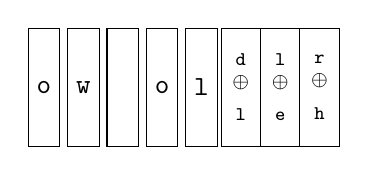
\begin{tikzpicture}[
   box/.style={rectangle,draw,minimum width=0.4cm,
    minimum height=1.5cm,inner sep=+0.1cm}
    ]
    
  % -- bottom row
  \node[box] at (1,0) (b7) {\tt o};
  \node[box] at (1.5,0) (b6) { \tt w};
  \node[box] at (2,0) (b5) {{\tt }};
  \node[box] at (2.5,0) (b4) {\tt o};
  \node[box] at (3,0) (b3) {\tt l};
  \node[box,text width=0.3cm,align=center] at (3.5,0) (b0) {\scriptsize \tt d \\ $\oplus$ \\ l};
  \node[box,text width=0.3cm,align=center] at (4,0) (b0) {\scriptsize \tt l \\ $\oplus$ \\ e};
  \node[box,text width=0.3cm,align=center] at (4.5,0) (b0) {\scriptsize \tt r \\ $\oplus$ \\ h};
  
\end{tikzpicture}
\end{center}
\end{example}

The following gives the {\tt C} code of the XOR wrap hash:
\begin{verbatim}
void hash(char* s, int len, uint64_t* hash_p)
  // takes string s of length <len> performs XOR wrap hash
{
  *hash_p = 0;
  int i = 0;
  int count_to_8 = 0; // to address the 8 byte-parts of uint64_t

  while (i < len)
  {
    *(hash_p) = *(hash_p) ^ (((uint64_t)(*s)) << (count_to_8 * 8));
    count_to_8++; 
    if (count_to_8 == 8)    // wrap!
      count_to_8 = 0;
    s++;
    i++;
  }
}
\end{verbatim}
% . . . . . . . . . . . . . . . . .
\section{Rolling XOR hash}
The whole point of the rolling XOR hash will be: we do not have
to always recalculate the XOR wrap hash of the text window. We 
can do this in a shorter manner that is {\em  
independent of the length of the pattern}.

The rolling XOR hash takes two ingredients:
\begin{enumerate}
    \item The simplicity of the XOR wrap hash, and 
    \item the fact that for $\oplus$, every element is its own inverse,
    that is, given  any bit-string $x$, we have $$x \oplus x = 0.$$
\end{enumerate}
Coming back to our {\tt hello world} example, we assume that 
the next character in the text window is {\tt `!'}. So
in order to ``get the hash rolling'', we need to delete the ``old''
character {\tt h} which drops out at the back (using XOR), and integrate
the new character {\tt `!'} into the hash (using XOR again!). 
So we perform the following  3 steps:
\begin{enumerate}
    \item {\bf Delete} {\tt h} using XOR at the least significant 8 bits of 
    {\tt h}.
    \item {\bf Right-rotate} {\tt h} by 8 bits. 
    \item {\bf Insert} new character with XOR at position {\tt len-1 \% 8}.
\end{enumerate}
Pictorially, the situation before the roll is:

\begin{center}
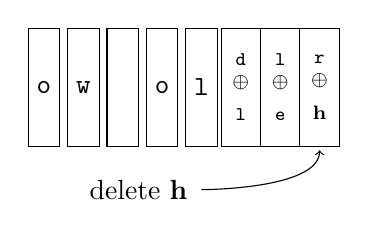
\begin{tikzpicture}[
   box/.style={rectangle,draw,minimum width=0.4cm,
    minimum height=1.5cm,inner sep=+0.1cm}
    ]
    
  % -- bottom row
  \node[box] at (1,0) (b7) {\tt o};
  \node[box] at (1.5,0) (b6) { \tt w};
  \node[box] at (2,0) (b5) {{\tt }};
  \node[box] at (2.5,0) (b4) {\tt o};
  \node[box] at (3,0) (b3) {\tt l};
  \node[box,text width=0.3cm,align=center] at (3.5,0) (b0) {\scriptsize \tt d \\ $\oplus$ \\ l};
  \node[box,text width=0.3cm,align=center] at (4,0) (b0) {\scriptsize \tt l \\ $\oplus$ \\ e};
  \node[box,text width=0.3cm,align=center] at (4.5,0) (b0) {\scriptsize \tt r \\ $\oplus$ \\ {\bf h}};
 
  
  % -- arrow
   \draw[->] (3,-1.3) .. controls (3,-1.3) and (4.5,-1.3) .. (4.5,-0.8);
   
  \node at (2.2,-1.3) {delete {\bf h}};
  
\end{tikzpicture}
\end{center}
After performing the three steps (delete / rotate / insert) above, we get

\begin{center}
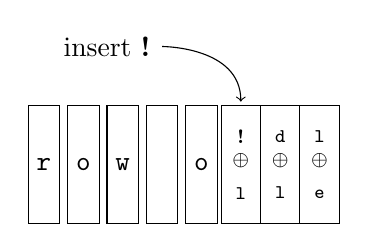
\begin{tikzpicture}[
   box/.style={rectangle,draw,minimum width=0.4cm,
    minimum height=1.5cm,inner sep=+0.1cm}
    ]
    
  % -- bottom row
  \node[box] at (1,0) (b7) {\tt r};
  \node[box] at (1.5,0) (b6) { \tt o};
  \node[box] at (2,0) (b5) {{\tt w}};
  \node[box] at (2.5,0) (b4) {\tt };
  \node[box] at (3,0) (b3) {\tt o};
  \node[box,text width=0.3cm,align=center] at (3.5,0) (b0) {\scriptsize \tt {\bf !} \\ $\oplus$ \\ l};
  \node[box,text width=0.3cm,align=center] at (4,0) (b0) {\scriptsize \tt d \\ $\oplus$ \\ l};
  \node[box,text width=0.3cm,align=center] at (4.5,0) (b0) {\scriptsize \tt l \\ $\oplus$ \\ e};
  
    % -- arrow
   \draw[<-] (3.5,0.8) .. controls (3.5,1.5) and (2.5,1.5) .. (2.5,1.5);
   
  \node at (1.8,1.5) {insert {\bf !}};
  
\end{tikzpicture}
\end{center}

The code for the rolling XOR hash is surprisingly short:

\begin{verbatim}
void hash_rolling(char delete_char, char add_char, int len, uint64_t* hash_p)
{
  *hash_p = *hash_p ^ (uint64_t)delete_char; // Delete
  uint64_t rightmost_byte = *hash_p & ((1 << 8) - 1); // Rotate
  *hash_p = (*hash_p >> 8) | (rightmost_byte << 56);
  *hash_p = *hash_p ^ ((uint64_t)add_char << ((len - 1) % 8 ) * 8);
                                   // Insert
}
\end{verbatim}

To summarize, the XOR wrap hash and the XOR rolling hash 
are used in the following manner: 
\begin{enumerate}
    \item Calculate XOR wrap hash of both pattern, and text window
    in initial position within text.
    \item Compare these hashes.
    \item Move window and calcuate rolling XOR hash. If at any state,
    the pattern hash and the window hash are equal, a match is declared 
    to be found.
\end{enumerate}
% . . . . . . . . . . . . . . . . .
%\section{Performance results}

%................... bibliography .................
{\footnotesize
\begin{thebibliography}{99}
%\bibitem{Er} \Erd, Paul, {\it On the combinatorial problems which I would
%most like to see solved}, Combinatorica {\bf 1} (1981), 25--42.
\bibitem{RK} Karp, Richard M., Rabin, Michael O.~(1987) ``{\it Efficient randomized pattern-matching algorithms}''. 
IBM Journal of Research and Development {\bf 31} (2): 249–260.
\end{thebibliography}
} %-- end footnotesize
\end{document}
